%!TEX root = ../thesis.tex
%*******************************************************************************
%****************************** Second Chapter *********************************
%*******************************************************************************

\chapter{Linear mixed models for quantitative genetics}

In chapters 4-6 I describe various models for eQTL mapping using single cell expression profiles. 
All of these models build on a linear mixed model framework. 
I use this chapter to provide an overview of linear and linear mixed models and their application in quantitative genetics, with a focus on their use for eQTL mapping. 
I will also introduce LMM-based models to test for GxE interactions, to provide the necessary theoretical foundations for the analyses in chapters 5 and 6.\\

Linear mixed models (LMMs) are a very popular framework for many genetic analyses. 
They are especially appealing because they provide robust control for confounding factors. 
While inference using LMMs is in general computationally demanding, there exist efficient implementations of specific LMMs, which enable applications to large datasets. 
In this chapter, I give an overview of the use of LMMs in genetic association studies and efficient algorithmic implementations. 
In sections 2.1-2.2, I discuss the linear model (also called linear regression) and basic applications for genome-wide association studies (GWAS) and quantitative trait loci (QTL) mapping. 
In section 2.3, I introduce the linear mixed model (LMM) and discuss applications in genetics, with a focus on the use of LMMs for expression-QTL (eQTL) mapping. 
Finally, in Section 2.4, I discuss extensions of the LMM framework to test for genotype-environment (GxE) interactions.\\

\newpage

For mathematical model descriptions throughout this thesis, I use the following notation: bold, small letters symbolise one-dimensional column vectors (e.g. $\mathbf{v}$) and bold capitalised letters matrices (e.g. $\mathbf{M}$). 
A normal distribution is specified by $ N(\mu, \sigma^2)$, where $\mu$, $\sigma$ are two scalars representing the mean and standard deviation parameters.
For simplicity, I use the same notation for multivariate normal (e.g. $ N(\boldsymbol{\mu}, \boldsymbol{\Sigma})$), noting that the specified parameters are a Nx1 mean vector, and a  NxN covariance matrix.

%********************************** %First Section  **************************************

\section{Linear regression} 

A linear model, or regression, is a statistical approach to modelling a continuous output variable (or outcome, dependent variable) as a linear function of one or more input variables (features, or independent variables). For F features, the outcome variable for a single individual i is:

\begin{equation} \label{eq1:Linear_regression_sample_i}
 y_i = \sum_{f=1}^{F} x_{i,f}\beta_i + \psi_i
\end{equation}

The noise term $\psi_i$ ($ \psi_i \sim N(0, \sigma_N^2)$) accounts for measurement noise of $y_i$, reflecting the non-deterministic relationship between $y_i$ and $x_{i,f}$, and is assumed to follow a Gaussian distribution with 0 mean and constant variance $\sigma_N^2$. Furthermore, the noise term is assumed to be independent across samples. For N samples, the model in (eq. 2.1) can be expressed in matrix form as:

\begin{equation} \label{eq2:Linear_regression_matrix_form}
\mathbf{y} = \mathbf{X}\boldsymbol{\beta} + \boldsymbol{\psi} 
\end{equation}

With $ \boldsymbol{\psi} \sim N(\mathbf{0}, \sigma_N^2 \mathbf{I_N})$, where $\mathbf{I_N}$ denotes the N x N identity matrix. \\ 

We can then write:

\begin{equation} \label{eq3:Linear_regression_MVN_form}
\mathbf{y} \sim N(\mathbf{X}\boldsymbol{\beta}, \sigma_N^2 \mathbf{I_N}) 
\end{equation}

\newpage

\subsection{Maximum likelihood solution}

Equation (2.3) is a direct representation of the probability distribution of the data $p(\mathbf{y}| \mathbf{X}, \boldsymbol{\beta}, \sigma_N^2)$ given the input variables $\mathbf{X}$ and the model parameters $\boldsymbol{\beta}$ and $\sigma_N^2$.
This probability is known as the likelihood of the model and, for parameter inference, is typically regarded as a function of the model parameters and denoted as $L(\boldsymbol{\beta}, \sigma_N^2)$. 
Thus, the model in (2.3) can be equivalently expressed as:\\

\begin{equation} \label{eq4:Linear_regression_likelihood}
 L(\boldsymbol{\beta}, \sigma_N^2) = p(\mathbf{y}| \mathbf{X}, \boldsymbol{\beta}, \sigma_N^2) = N(\mathbf{y} | \mathbf{X}\boldsymbol{\beta}, \sigma_N^2 \mathbf{I}) 
\end{equation}

The log marginal likelihood of the model can be explicitly specified as:\\

\begin{equation} \label{eq5:Linear_regression_log_likelihood}
\begin{split}
logL(\boldsymbol{\beta}, \sigma_N^2) = -\frac{1}{2} \bigg\{Nlog(2\pi)\sigma_N^2) + log|I| \frac{1}{\sigma_N^2}(\mathbf{y}-\mathbf{X}\boldsymbol{\beta})^T\mathbf{I_N}^{-1}(\mathbf{y}-\mathbf{X}\boldsymbol{\beta}) \bigg\}  = \\
= -\frac{N}{2}log(2\pi)) - \frac{N}{2}log(2\pi))- 0 - \frac{1}{2\sigma_N^2}(\mathbf{y}-\mathbf{X}\beta)^T(\mathbf{y}-\mathbf{X}\beta)  
\end{split}
\end{equation}

The maximum likelihood estimator (MLE) of the model parameters is defined as the set of parameter values that maximise the likelihood (or its log). Denoting with $\hat{\boldsymbol{\beta}}$ and $\hat{\sigma_N^2}$ the MLE of $\boldsymbol{\beta}$ and $\sigma_N^2$ we can write:

\begin{equation} \label{eq6:Linear_regression_MLEs}
\hat{\boldsymbol{\beta}},\hat{\sigma_N^2} = argmax_{\boldsymbol{\beta},\sigma_N^2}L(\boldsymbol{\beta}, \sigma_N^2) 
\end{equation} 

By setting the gradient of the log likelihood in (2.5) with respect with both parameters to zero, and solving the joint system:

\begin{equation} \label{eq7:Linear_regression_MLE_system}
\systeme{
    \dfrac{\partial logL(\boldsymbol{\beta}, \sigma_N^2)}{\partial \boldsymbol{\beta}} = \mathbf{0},
    \dfrac{\partial logL(\boldsymbol{\beta}, \sigma_N^2)}{\partial \sigma_N^2} = 0
    }
\end{equation}

We find:

\begin{equation} \label{eq8:Linear_regression_MLE_solution_beta}
\hat{\boldsymbol{\beta}} = (\mathbf{X}^T\mathbf{X})^{-1}\mathbf{X}^T\mathbf{y} 
\end{equation}

\begin{equation} \label{eq9:Linear_regression_MLE_solution_sigma}
 \hat{\sigma_n^2} = \frac{1}{N}(\mathbf{y}-\mathbf{X}\hat{\boldsymbol{\beta}})^T(\mathbf{y}-\mathbf{X}\hat{\boldsymbol{\beta}}) = \frac{1}{N}(\mathbf{y}-\mathbf{X}(\mathbf{X}^T\mathbf{X})^{-1}\mathbf{X}^T\mathbf{y})^T(\mathbf{y}-\mathbf{X}(\mathbf{X}^T\mathbf{X})^{-1}\mathbf{X}^T\mathbf{y}) 
\end{equation}

Note that the solution for $\hat{\boldsymbol{\beta}}$ (eq 2.8) is equivalent to the ordinary least squares (OLS) solution (ref).


\subsection{Restricted maximum likelihood}

In Gaussian models as in (2.3) the MLE of the variance parameter $\hat{\sigma_N^2}$ is biased because the weights $\hat{\boldsymbol{\beta}}$ are estimated from the data, which entails a reduction of the effective number of degrees of freedom.
Patterson and Thompson (1971) proposed a solution to $\boldsymbol{\beta}$-free estimation of $\sigma_N^2$ via the restricted (or residual) maximum likelihood (REML).

Given (2.2) REML can be obtained by projecting the output vector in a space that is orthogonal to $\mathbf{X}$:

\begin{equation}
    \mathbf{A}\mathbf{X} = \mathbf{0}
\end{equation}

Using (2.10) and rewriting (2.3) in terms of the projection $\mathbf{w}$ we obtain:

\begin{equation}
    \mathbf{w} = \mathbf{A}\mathbf{y} = \mathbf{A}(\mathbf{X}\boldsymbol{\beta} + \boldsymbol{\psi}) = \mathbf{A}\boldsymbol{\psi}
\end{equation}

which provides an expression of $\mathbf{y}$ that is independent of $\boldsymbol{\beta}$.\\

By estimating $L(\sigma_N^2 | \mathbf{A}\mathbf{y} )$ for the model in (eq. 2.3), we obtain the following log restricted maximum likelihood:

\begin{equation} \label{eq10:Linear_regression_log_restricted_likelihood}
\begin{split}
logL(\sigma_N^2) = -\frac{N-F}{2}log(2\pi) - \frac{1}{2}log|\mathbf{X}^T\mathbf{X}| \\
-  \frac{N-F}{2}log\sigma_N^2 - \frac{1}{2\sigma_N^2}(\mathbf{y}-\mathbf{X}\hat{\boldsymbol{\beta}})^T(\mathbf{y}-\mathbf{X}\hat{\boldsymbol{\beta}})  
\end{split}
\end{equation}

which is maximised by

\begin{equation}\label{eq11:Linear_regression_REML_sigma}
\hat{\sigma_n^2}_{REML} =  \frac{1}{N-F}(\mathbf{y}-\mathbf{X}(\mathbf{X}^T\mathbf{X})^{-1}\mathbf{X}^T\mathbf{y})^T(\mathbf{y}-\mathbf{X}(\mathbf{X}^T\mathbf{X})^{-1}\mathbf{X}^T\mathbf{y})
\end{equation}

Eq. (2.13) is identical to eq. (2.9) with the exception that N is replaced by (N - F), which denotes the loss of F degrees of freedom.

%********************************** %Second Section  **************************************

\section{Linear models for association studies}

When applyinh linear models in genetic association studies, the outcome variable ($\mathbf{y}$) is a phenotype, that is a measurable characteristic of the samples considered. 
In GWAS, we typically look at "global phenotypes".
These can be traits such as height and eye colour or disease status/risk for various illnesses (such as diabetes, or rheumatoid arthritis, see \textbf{Section 1.1.y} of the Introduction).
In QTL mapping, we consider "molecular phenotypes". 
Those can be quantification of molecular traits such as gene expression (i.e. eQTL), or protein level (pQTL), etc. (\textbf{Section 1.2.x}).
The test then consists in assessing the effect of single nucleotide polymorphisms (SNPs),  onto such phenotype. 
We test the effect of one SNP ($\mathbf{g}$) at the time, and assume all SNPs to be biallelic, that is that they can only assume two possible values. 

\begin{equation}\label{eq12:Linear_regression_genetics}
 \mathbf{y} = \mathbf{g}\beta + \boldsymbol{\psi} 
\end{equation}

Let us consider a bi-allelic variant with major allele a and minor allele A. 
For the minor allele A, we can consider either a dominant model (aa = 0, Aa = 1, AA = 1; where only one copy of the allele is necessary to have a phenotypic effect), a recessive model, (aa = 0, Aa = 0, AA = 1; where two copies of the minor allele must be present for a phenotypic effect) or an additive model (aa = 0, Aa = 1, AA = 2; where the effect is proportional to the minor allele count). 
In this thesis, we will consider an additive genetic model, which is widely-used in the analysis of complex traits.

\subsection{Traits with binary outcomes}

It is worth noting that linear regressions are well suited for continuous traits, that can be approximated to follow a normal distribution. 
Another widely used model for genetic analyses is the logistic regression (or logit regression), where a logit function is applied to a linear predictor ($\mathbf{z}$) to better reflect the data in case of binary outcomes ($\mathbf{y}$). 
This is very often used when the phenotype of interest reflects the presence or absence of a certain disease (so called case/control studies).
In this case, the outcome can be thought of in terms of sampling from a binomial distribution, with a fixed number of samples N, and a probability p to have the disease. Then, the model becomes:

\begin{equation}\label{eq13:Logistic_regression_genetics_z}
 logit(\mathbf{y}) = \mathbf{z} = \mathbf{g}\beta + \boldsymbol{\psi} 
\end{equation}

Logistic regressions are a particular example of a larger class of models, the generalised linear models (GLMs). 
GLMs are used when the distribution of the outcome variable cannot be approximated to a Gaussian distribution. 
In the example above, a logit distribution is better suited to model a binary variable. 
In other cases, we might have count data better approximated by a Poisson distribution, etc.
The three requirements of a GLM are i) to have a linear predictor ($\mathbf{z}$), ii) that the distribution of $\mathbf{y}$  belongs to the exponential family (\textbf{Box 2}), and iii) that we can define a link function $g$ such that, similar to above:

\begin{equation*}
 E[\mathbf{y}] = g(\mathbf{z})^{-1} 
\end{equation*}

In eq. (2.13), $ g = logit $.


%****** Box on exponential family distributions ******

\newpage

\begin{Comment}
\hspace{-2.5mm}\textbf{Box 2: Exponential Family distributions}\label{box2}\\
% \small
In probability and statistics, an exponential family is a parametric set of probability distributions of the form:

\begin{equation*}
    p(x) = h(x)e^{\theta^TT(x)-A(\theta)}
\end{equation*}

Members of the exponential family distributions include:
\begin{itemize}
    \item Normal distribution: $X \sim N(\mu,\sigma^2)$
    \item Exponential distribution: $ X \sim Exp(\lambda)$
    \item Gamma distribution: $ X \sim \Gamma(\alpha,\beta)$
    \item Chi-squared distribution: $ X \sim \chi^2 (k)$ or $ X \sim \chi_k^2$
    \item Beta distribution: $ X \sim Beta(\alpha,\beta)$
    \item Dirichlet distribution: $ X \sim Dir(\alpha)$
    \item Bernoulli distribution: $ X \sim Be(p)$ or $ X \sim Bernoulli(p)$
    \item Poisson distribution: $ X \sim P(\lambda)$ or $ X \sim Pois(\lambda)$
    \item Binomial distribution (with fixed number of trials): $ X \sim B(n,p)$
    \item Negative Binomial distribution (with fixed number of failures): $ X \sim NB(r,p)$\\
\end{itemize}

For example, take the Bernoulli case: $x \in X \sim Be(p)$:

\begin{equation*}
\begin{split}
    p(x) & = p^x(1-p)^{(1-x)}\\
         & = e^{log(p^x(1-p)^{(1-x)})}\\
         & = e^{xlogp + (1-x)log(1-p)}\\
         & = e^{xlog\frac{p}{1-p}+log(1-p)}\\
         & = e^{x\theta - log(1+e^\theta)}
\end{split}
\end{equation*}

where: 

\hfill $h(x)=1 \hfill T(x)=x \hfill \theta = log \frac{p}{1-p} \hfill A(\theta) = log(1+e^\theta)$ \hfill

\end{Comment}

%**************

\newpage

\subsection{Statistical hypothesis testing}

To test for whether an association between a genetic variant and a trait is present, we can compare the hypothesis where the genetic variant has no effect on the trait (called null hypothesis, $H_0$) and the alternative hypothesis when the variant does have an effect (effect different from 0, $H_1$).
Formally, the association hypothesis test is:

\begin{equation}\label{eq14:null_hypothesis}
 H_{0}: \beta=0 
\end{equation}
vs
\begin{equation}\label{eq15:alternative_hypothesis}
 H_{1}: \beta \neq 0 
\end{equation}

We are then comparing the following models (from eq. 2.14):

\begin{equation}\label{eq16:null_hypothesis_regression}
 H_0: \mathbf{y} \sim N(\mathbf{0}, \sigma_N^{2} \mathbf{I_N}) 
\end{equation}

\begin{equation}\label{eq17:alternative_hypothesis_regression}
 H_1: \mathbf{y} \sim N(\mathbf{g}\beta,\sigma_N^{2} \mathbf{I_N}) 
\end{equation}

Statistical hypothesis testing consists of three fundamental steps: 1) define a test statistic; 2) obtain a P-value and 3) upon a threshold on the P-value, reject or accept the null hypothesis. 
A test statistic is a random variable that quantifies the difference between the null hypothesis $H_0$ and what is observed in the sample. 
Once we have a test statistic, we calculate a probability value ("P value") as the probability, under the null hypothesis $H_0$, of sampling a test statistic at least as extreme as the observed one. 
An extreme value of the test statistic generally indicates evidence against $H_0$.
The P value is a function of the test statistic and, by definition, it is uniformly distributed under $H_0$.
Finally, if this probability is low (under a defined threshold, e.g. P < 0.05) $H_0$ is rejected and $H_1$ accepted (positive result).
Otherwise, we reject $H_1$ and accept $H_0$ (negative result).\\

In statistical hypothesis testing, two types of errors can be made. 
We can either reject $H_0$ when $H_0$ is true, thus generating a false positive (type I error), or reject $H_1$ when $H_1$ is true, generating a false negative (type II error).
Other concepts that are central to statistical hypothesis testing are the significance level, defined as the type I error rate (i.e. the expected percentage of false positives), and the statistical power, which is the true positive rate under $H_1$ (i.e. the ability to recover true associations, \textbf{Box 3}).

%****** Box on confusion matrix ******

\newpage

\begin{Comment}
\hspace{-2.5mm}\textbf{Box 3: Key concepts of statistical testing}\label{box3}\\
% \small
Confusion matrix:

\begin{center}
\begin{tabular}{l|l|c|c|}
\multicolumn{2}{c}{}&\multicolumn{2}{c}{Test Result}\\
\cline{3-4}
\multicolumn{2}{c|}{}&reject $H_0$&accept $H_0$\\
\cline{2-4}
\multirow{2}{*}{Actual value}& $H_1$ & True Positive ($TP$) & False Negative ($FN$)\\
\cline{2-4}
& $H_0$ & False Positive ($FP$) & True Negative ($TN$)\\
\cline{2-4}
\end{tabular}
\end{center}

\begin{itemize}
    \item Type I error $= FP$
    \item Type II error $= FN$
    \item Sensitivity $=$ Recall $=$ True positive rate (TPR) $=$ Power $=\frac{TP}{TP+FN}$
    \item Specificity $=$ True negative rate (TNR) $=\frac{TN}{TN+FP}$
    \item False positive rate (FPR) $= 1-$Specificity $=$ Size $=\frac{FP}{TN+FP}$
    \item Precision $=$ Positive predictive value (PPV) $=\frac{TP}{TP+FP}$
    \item Accuracy $=\frac{TP+TN}{TP+TN+FP+FN}$
    \item $F_1$ score $F_1=2 \frac{PPV*TPR}{PPV+TPR}=\frac{2TP}{2TP+FP+FN}$
    \item Family-wise error rate (FWER) $=P(FP \geq 1)= 1 - P(FP=0)$
    \item False discovery rate (FDR) $=\frac{FP}{TP+FP}= 1- $Precision
\end{itemize}

\vfill

\end{Comment}

%**************

\vspace{5mm}

Three approaches are commonly used for statistical testing in genetic association analyses: the Wald test, the likelihood ratio test (LRT), and the score test (\textbf{Fig. 2.1}).
In the next paragraphs, I will describe briefly all three but focusing on the two latter ones, which are used in this thesis.

\begin{figure}[h]
\centering
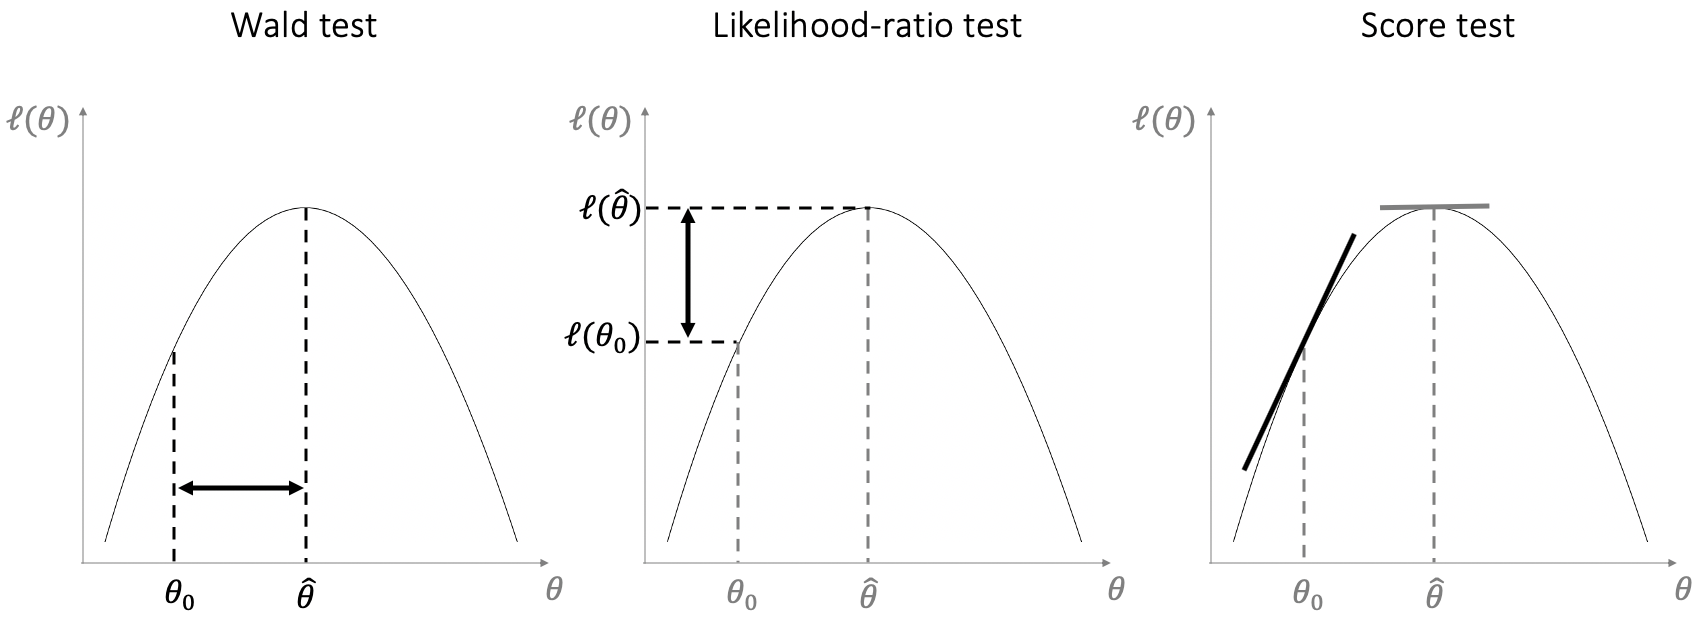
\includegraphics[width=15cm]{Chapter2/Fig/wald_lrt_score_tests.png}
\caption{\textbf{The Wald test, the likelihood-ratio test and the score test}.\\
The three most commonly used statistical testing approaches are illustrated here in the univariate case (single parameter $\theta$). 
On the x axis is the parameter $\theta$ on the y axis the log likelihood $\mathit{l}(\theta)$.
The Wald test essentially evaluates the difference between the MLE $\hat{\theta}$ and the parameter under $H_0$, $\theta_0$.
The likelihood-ratio test evaluates the difference between the log likelihoods evaluated at those values, i.e. $\mathit{l}(\hat{\theta})$ and $\mathit{l}(\theta_0)$.
Finally, the Score test evaluates the slope of $\mathit{l}(\theta)$ at $\theta_0$. Note that the slope at $\hat{\theta}=0$ by definition, as the MLE maximises $\mathit{l}(\theta)$.}
\end{figure}

\subsubsection{Wald test}

First, let us consider the Wald test and let us consider the generic null hypothesis $H_0: \boldsymbol{\theta} = \boldsymbol{\theta}_0$ and the alternative $H_1: \boldsymbol{\theta} \neq \boldsymbol{\theta}_0$.
The Wald test statistic is defined as:

\begin{equation}
W = (\hat{\boldsymbol{\theta}}-\boldsymbol{\theta_0})^T [var(\boldsymbol{\theta_0})]^{-1}(\hat{\boldsymbol{\theta}}-\boldsymbol{\theta_0}) 
\end{equation}

Under some assumptions (ref), $W$ follows a chi-squared ($\chi^2$) distribution with number of degrees of freedom (dof) $d$ equal to the number of tested parameters ($W \sim \chi^2_d $).\\

In the univariate case (d = 1), eq (2.20) can be expressed as:

\begin{equation}
    W = \frac{(\hat{\theta}-\theta_0)^2}{var(\hat{\theta})} \sim \chi^2_1
\end{equation}

Intuitively, the chance of rejecting $H_0$ increases as $\hat{\theta}$ is further away from $\theta_0$ and decreases as our confidence ... (i.e. $var(\theta_0)$ increases).


\subsubsection{Likelihood ratio test}

Second the likelihood ratio test (LRT).
It was first introduced by XX. 
The test statistic in this case is the (log) likelihood ratio ($LLR$):

\begin{equation}\label{eq18:log_likelihood_ratio}
LLR = log \frac{L(H_1)}{L(H_0)} = logL(H_1) - logL(H_0) 
\end{equation}

Where we compare the value of the log-likelihood of the model under $H_0$ and $H_1$, by evaluating eq. 2.5 (or 2.12) using MLE parameters estimated under $H_0$ ($\mathbf{0}$, $\sigma_0^2$) or $H_1$ ($\hat{\boldsymbol{\beta}}$, $\hat{\sigma_1^2}$).  \\

Similarly to the Wald test, in this case the Wilks theorem (1938),under some assumptions, guarantees that $2LLR$ follows a chi-squared ($\chi^2$) distribution with $d$ dof ($2LLR \sim \chi^2_d$).

The P-value can be calculated as:

\begin{equation}
    P(LLR) = 
\end{equation}

\subsubsection{Score test}

Finally the score test, also known as Lagrange multiplier test, is the last hypothesis test we consider. 
It was first developed by Rao in 1948 (\cite{rao1948large}).
First, we define the score vector of Fisher:

\begin{equation}
    \mathbf{S} = \frac{\partial L}{\partial \boldsymbol{\theta}}
\end{equation}

The Score test statsitic is the Lagrange Multiplier (LM):

\begin{equation}
    LM = \mathbf{S}(\boldsymbol{\theta_0})^T [var(\boldsymbol{\theta_0})]^{-1}\mathbf{S}(\boldsymbol{\theta_0}) 
\end{equation}

It can be shown that this, too follows a chi-squared distribution with $d$ dof ($LM \sim \chi^2_d$).

To understand the intuition behind this test let us consider again the univariate case (d = 1):

\begin{equation}
    LM = \frac{S(\theta_0)^2}{var(\theta_0)} \sim \chi^2_1
\end{equation}

At the MLE $\hat{\theta}$, the log likelihood and therefore its gradient $S(\hat{\theta})$ is equal to 0.
On the contrary, in principle, $ S(\theta_0) \neq 0 $. 
Intuitively, the further away from 0, the more likely we are to reject the null hypothesis.
Fast methods to infer the p-value of a Score test were proposed by Davies exact method \cite{davies1980algorithm} and Liu:

\begin{equation}
    P(Q<c)
\end{equation}


\subsubsection{Intuition on differences between LRT and score test}

In this thesis, we apply both the LRT and the Score test, for different applications.
I use this paragraph to highlight the key differences between the two tests and provide an intuition as to when one should use one or the other.\\

First of all, it can be shown that (finite sample, ref):

\begin{equation}
    W \geq LLR \geq LM
\end{equation}

Let us exclude the Wald test for this purposes, eq (2.28) guarantees that the log-likelihood ratio is always greater than the Lagrange multiplier.
As a consequence, the power (\textbf{Box 3}) of the LRT, defined as the probability of rejecting the null hypothesis when it is false: $P = P($reject $H_0 | H_1)$ is higher than the power of the Score test.

\begin{equation}
    (P_W \geq) P_{LLR} \geq P_{LM}
\end{equation}

On the other hand, the size (\textbf{Box 3}) of the LRT, defined as the probability of rejecting the null hypothesis when it is true: $S = P($reject $H_0 | H_0)$ is also higher than the size of the Score test.
The Score test is therefore more accurate, making a smaller (or equal) number of Type I error. The LRT is robust to re-parametrization of the parameters, whereas the score test (or the Wald test) is not. On the other hand, one main advantage of the Score test is that we do not actually evaluate the MLE of the parameters, but only evaluate the likelihood under the null.
Finally, the LLR follows a chi-squared distribution (asymptotically) only under the assumptions of the Wilks' theorem, which can be violated in certain applications.
Namely, the value of parameters tested should be far away from the boundaries of the possible values the parameter can assume.
For example, $-\infty < \beta < \infty$, so testing $H_1: \beta \neq 0$ satisfies the assumption.
On the other hand, $0 < \sigma^2 < \infty$ so testing $H_1: \sigma^2 \neq 0$ violates the assumption, because the value $0$ is right at the boundary.\\

I will use the LRT in the analyses in chapters 4 and 5, where the tests evaluate $\boldsymbol{\beta}$.
I use Rao's score test in chapter 6, where I will be evaluating the variance parameter $\sigma^2$.


\subsection{Multiple Testing Correction}

Hundreds of thousands or millions of variants may be individually tested within a typical human GWAS. 
In eQTL mapping, we might test tens of thousands of genes, each essentially equivalent to a GWAS trait. 
Even when we only test for \textit{cis} eQTL, we will still test hundreds of variants per gene, bringing the average number of tests performed well over 10 Millions [REF].  
When performing such a large number of tests, controlling single test P values results in a high number of false positives (for example, for P < 0.01 and 10$^6$ tests we expect 10,000 false positives under the null hypothesis). 
This problem is known as the multiple hypothesis testing problem. 
In the next paragraphs, I give a brief overview of the methods commonly used in genetic analysis to correct for multiple hypothesis testing, with a focus on methods used in eQTL mapping.

\subsubsection{Controlling family-wise error rate} 

One strategy to perform multiple testing correction is to control the probability of having at least one false positive in the experiment, which corresponds to an experiment-wise P value known as family-wise error rate (FWER, \textbf{Box 3}).
The widely used Bonferroni method follows this strategy assuming independence between tests. 
Given a desired family-wise significance level $\alpha$, the method consists in calculating adjusted P values as $P_{adj} = P*n $, where n is the number of tests, and setting $P_{adj} < \alpha$ . 
This strategy ensures FWER < $\alpha$. 
The Bonferroni correction strategy is conservative, because of the assumption of independence between tests, which ignores correlations between genotypes due to linkage disequilibrium (LD).\\

An alternative strategy, which accounts for the dependency of the statistical tests, is to consider permutations. 
For example, one way to control the FWER by using permutations is to perform the experiment M times, each time considering a different permutation of the genotype data across individuals.
The minimum P values from these M additional experiments are then used to calculate an experiment-wise P value, as the fraction of the M minimum permutation P values that are lower than the minimum observed P value. 

For test i, the adjusted P value after m permutations is calculated as:

\begin{equation}\label{eq19:permutation_adjusted_pvalue}
    P_{adj,i}^{perm} = \frac{1+\sum_{m=1}^{M} q_{i,m} \geq P_i}{1+M}
\end{equation}

Where $q_{i,m}$ is the P value obtained at the m$^{th}$ permutation run equivalent to test i, and ones are added to avoid zero divisions.  
This strategy accounts for local LD, thereby increasing the statistical power, and has been widely used in $cis$ molecular QTL mapping to estimate gene-level P values (Sudmant et al., 2015; GTEx Consortium, 2015).  

% rephrase this
However, as evident from eq. 2.30, a potentially very large number of permutations is needed to be able to detect a range of effects.
For example, for M=1,000 the smallest adjusted P value we can obtain is only $P_{adj}$=0.001 (when no permuted P value is smaller than the P value observed) which makes it hard to differentiate between more or less strong effects.
Additionally, in eQTL mapping a second round of multiple testing correction is necessary, across all genes so having smaller Ps would be beneficial.
For some applications, M should be as large as 100,000, which entails a great computational burden and can become unpractical in molecular analyses of large cohorts.\\

Recently, one method has been developed that uses permutation results for as little as (M=) 50-100 permutations to estimate a full distribution of background permuted P values, allowing to exploit the benefits of the assumption-free permutation approach without too much of the computational burden. 
This is the method I will use throughout this thesis to control for FWER at gene-level when performing large scale eQTL mapping.

\subsubsection{Controlling false discovery rate}

An alternative solution is to control the false discovery rate (FDR), i.e. the expected percentage of false discoveries (\textbf{Box 3}).
The most widely used FDR-based correction method is the Benjamini-Hochberg (BH) procedure (1995), which again assumes independence between tests. 
Let us consider T tests with P values $p_1, p_2, ..., p_T$ and let $r_1, r_2, ..., r_T$ be their ranks (the smallest P value has rank 1, the highest has rank T), defining adjusted P values as $P_{adj,i} = \frac{T*p_i}{r_i} $ and setting $P_{adj,i} <\alpha$ ensures FDR < $\alpha$.
In alternative, the Storey procedure (2002) is very similar to BH, but..

\subsubsection{Multiple testing correction for \textit{cis} eQTL mapping}

A typical strategy to correct for multiple hypothesis testing in molecular \textit{cis}-QTL mapping is to use a two-step procedure (Battle et al., 2014; Sudmant et al., 2015; GTEx
Consortium, 2015). 
First, for each gene an experiment-wise P value is obtained by correcting for multiple testing across variants using a FWER-based method. 
These gene-level P values are probability values for the hypothesis of a gene having at least
one QTL in the analysed region. 
Second, the gene-level P values are corrected to control the FDR, typically using the Benjamini-Hochberg procedure.\\

In this thesis, I adopt this two step approach.
I use M=1,000 permutations and the method described in [] to correct P values at the gene level (I will call the P values obtained this way "empirical feature P values").
Then, I select the top SNP per gene and correct the corresponding empirical feature P values a second time, using the Storey procedure ().
I will call the resulting P-values: "globally corrected P values".

\subsection{Accounting for confounding effects in linear model}

The model in eq. 2.14 assumes that the SNP tested is the only factor affecting the measured phenotype.
In reality often, if additional relevant information is available for the samples tested, such as sex or age, those can be added to the model as covariates $\mathbf{W}$:

\begin{equation}\label{eq21:Linear_regression_genetics_covariates}
 \mathbf{y} =  \mathbf{W}\boldsymbol{\alpha} + \mathbf{g}\beta + \boldsymbol{\epsilon} 
\end{equation}

Those are known as fixed effect (FE) covariates, and they only contribute to the mean of $\mathbf{y}$, such that $E[\mathbf{y}] = \mathbf{W}\boldsymbol{\alpha} + \mathbf{g}\beta$, while $Cov(\mathbf{y}) = Cov(\boldsymbol{\epsilon}) = \sigma_N^2 \mathbf{I_N} $, as before.
In some cases, we can use fixed effect covariates for other confounding, such technical batches and other experimental conditions that might skew the results. \\

In eQTL mapping, we can often take advantage of the expression profiles across all genes to identify global confounding affecting the expression of genes, even when we don't necessarily know the origin of the confounding.
For example, we can compute principal component analysis (PCA) on the full expression matrix (genes x samples) and include the first 5, 10 or 50 PCs as covariates in the model.
Alternative more sophisticated methods to compute factor capturing global trends are probabilistic estimation of expression residuals (PEER) \cite{stegle2010bayesian, stegle2012using} and multi-omics factor analysis (MOFA) \cite{argelaguet2018multi}. 

\subsection{Calibration studies and distributions on P-values}

Under the assumption of no association between genetic variants and the analysed trait, an association model is expected to produce approximately uniform P values.
If that is the case, the model is said to be calibrated.
To verify that a model is calibrated we can disrupt the association between genotypes and phenotypes, typically by shuffling the genotypes. 
A representation that is typically used to compare the observed (shuffled) and the expected distributions of P values is the quantile-quantile plot (QQ plot). 
In a QQ plot the observed -log10P is plotted against the expected -log10P, where the expected value is obtained from the uniform distribution. 
As confounding factors may create spurious associations, inflated QQ plots are typically associated with the presence of confounding and can be used as a diagnostic tool (Voight and Pritchard, 2005; Lin and Sullivan, 2009). 

% add figure here

%********************************** %Third Section  **************************************

\section{Population structure and linear mixed models}

A major source of confounding in genetic analysis that I have purposefully left out so far is population structure.
It was acknowledged, even before the first GWAS was conducted, that there was a possibility of identifying false positives (or that true positives may be masked) when using population based association studies instead of family based linkage studies, due to confounding effects (ref). 
This is due to the fact that both phenotypic prevalence (proportion of individuals exhibiting the phenotype) and allele frequencies (frequency of a specific allele within a population) vary across different populations, which may result in the identification of variants that are indirectly associated with the phenotype of interest due to ethnicity or population sub-structure (ref).

% name examples

\subsection{Approaches to account for pop struct}

Because we typically do not know the underlying sub-population structure of our samples, and therefore which specific genetic variants have different allele frequencies between such groups (and considering that it may be a relatively large number of such variants) we cannot directly include such variants as covariates (i.e. in $W$ from eq. 2.31).

Instead, various approaches have been proposed:

STRUCTURE (does not scale)

PCs (don't detect subtle relatedness effects)

LMMs (more computationally demanding but better)
it has been shown to perform exactly as well as regressing out (or including as covariates) all PCs, which is of course not feasible in practice. 

\subsection{Linear mixed models}

It will then introduce the use of random effect (RE) terms, making the transition from linear models to linear mixed models (LMMs). 
In equation 3,  is a random variable used to account for population structure; note that in all three cases, we test whether..

\begin{equation}\label{eq22:Linear_mixed_model}
 \mathbf{y} =  \mathbf{W}\boldsymbol{\alpha} + \mathbf{g}\beta + \mathbf{u} + \boldsymbol{\psi} 
\end{equation}

$\mathbf{u} \sim N(\mathbf{0}, \sigma_g^2\mathbf{K})$



GRM: genomic relationship matrix

\begin{equation}
    GRM = \frac{1}{N}\mathbf{X}\mathbf{X}^T
\end{equation}{}

plink (Purcell)

\subsection{Fast implementation of LMMs}

FaST-LMM, BOLT-LMM, LIMIX.


\subsection{LMMs for eQTL mapping}

It will conclude with a focus on the application of linear mixed models to eQTL mapping, making a distinction between cis and trans models and providing an overview of both alternative methods for eQTL mapping and large consortia and studies performing eQTL mapping.

%********************************** %Fourth Section  **************************************

\section{LMM for GxE (and StructLMM)}

As described in \textbf{Section 1.X}, GxE is defined as .. (Fig.)

Explicitly, whilst a variant with a significant genetic effect is determined by a mean phenotypic difference between groups of individuals with different allele dosages and a significant environment effect is determined by a mean phenotypic shift that is constant across different allele dosages (Fig. 1.6b), a significant statistical interaction effect is defined when there is a significant difference in the genetic effect between two groups of individuals with different environmental exposures.

\subsection{Stratified interaction test}

A possible way to detect interaction effects, is to stratify samples into discrete subgroups based on their environmental exposure.
Then a LM (eq. 2.31) or LMM (eq. 2.32) is applied to each strata and the marginal variant effects are compared to assess whether there is a significant difference in these effects across the sub-populations.
I will refer to this method as the "stratified interaction test" (ref).

For example different tissue / cell types

refer to GTEx

However, as more detailed environmental data is collected, allowing for finer stratification of the population, these methods are no longer optimal as the subpopulations become too small to obtain stable estimates of the variant effects.

\subsection{Single environment interaction test}

A second commonly used method to test for interaction effects is an extension of the LM or LMM to include two additional FE terms, an interaction term (GxE) and an environment term (E):

\begin{equation}\label{eq22:Interaction_test_FE_LMM}
 \mathbf{y} =  \mathbf{W}\boldsymbol{\alpha} + \mathbf{e}\gamma  + \mathbf{g}\beta_G + \mathbf{e}*\mathbf{g}\beta_{GxE} + \mathbf{u} + \boldsymbol{\epsilon} 
\end{equation}

\begin{equation}
 H_{0}: \beta_{GxE}=0 
\end{equation}
vs
\begin{equation}
 H_{1}: \beta_{GxE} \neq 0 
\end{equation}

\newpage

\subsection{StructLMM}

\begin{equation}\label{eq23:StructLMM-int}
 \mathbf{y} =  \mathbf{W}\boldsymbol{\alpha} + \mathbf{g}\beta_G + \mathbf{g} \otimes \boldsymbol{\beta_{GxE}} + \mathbf{e} + \boldsymbol{\epsilon} 
\end{equation}

% \section{Thesis outline}